\hypertarget{background}{\section{Background}}
\label{sec:background}
To begin, we provide a brief primer on the three core concepts underlying this work: foundation models, transparency, and indexes. 

\hypertarget{fms}{\subsection{Foundation models}}
\label{sec:background-fms}
Foundation models are the defining paradigm of modern AI, 
reflecting a broad shift in the field from bespoke models for individual tasks to more general models that can be adapted for a wide range of use cases \cite{bommasani2021opportunities}.
In this sense, foundation models belong to the broader class of general-purpose technologies that have restructured society such as electricity, the Internet, and smartphones \citep{bresnahan1995gpt, brynjolfsson2021jcurve, bommasani2021opportunities, eloundou2023gpts}. Building foundation models requires significant resources: immense volumes of data are processed using immense amounts of computation to yield the foundation model.
Using foundation models often requires substantially fewer resources in comparison: models can be adapted, often in lightweight fashion (\eg through a simple textual interface), for an increasingly wide range of use cases.
The disparity in resource requirements between development and deployment has yielded a market where a small set of companies build the most prominent foundation models that are then adopted by thousands of companies and millions of consumers \citep{bommasani2023ecosystem, vipra2023concentration, widder2023open}. 

\begin{figure}
\center
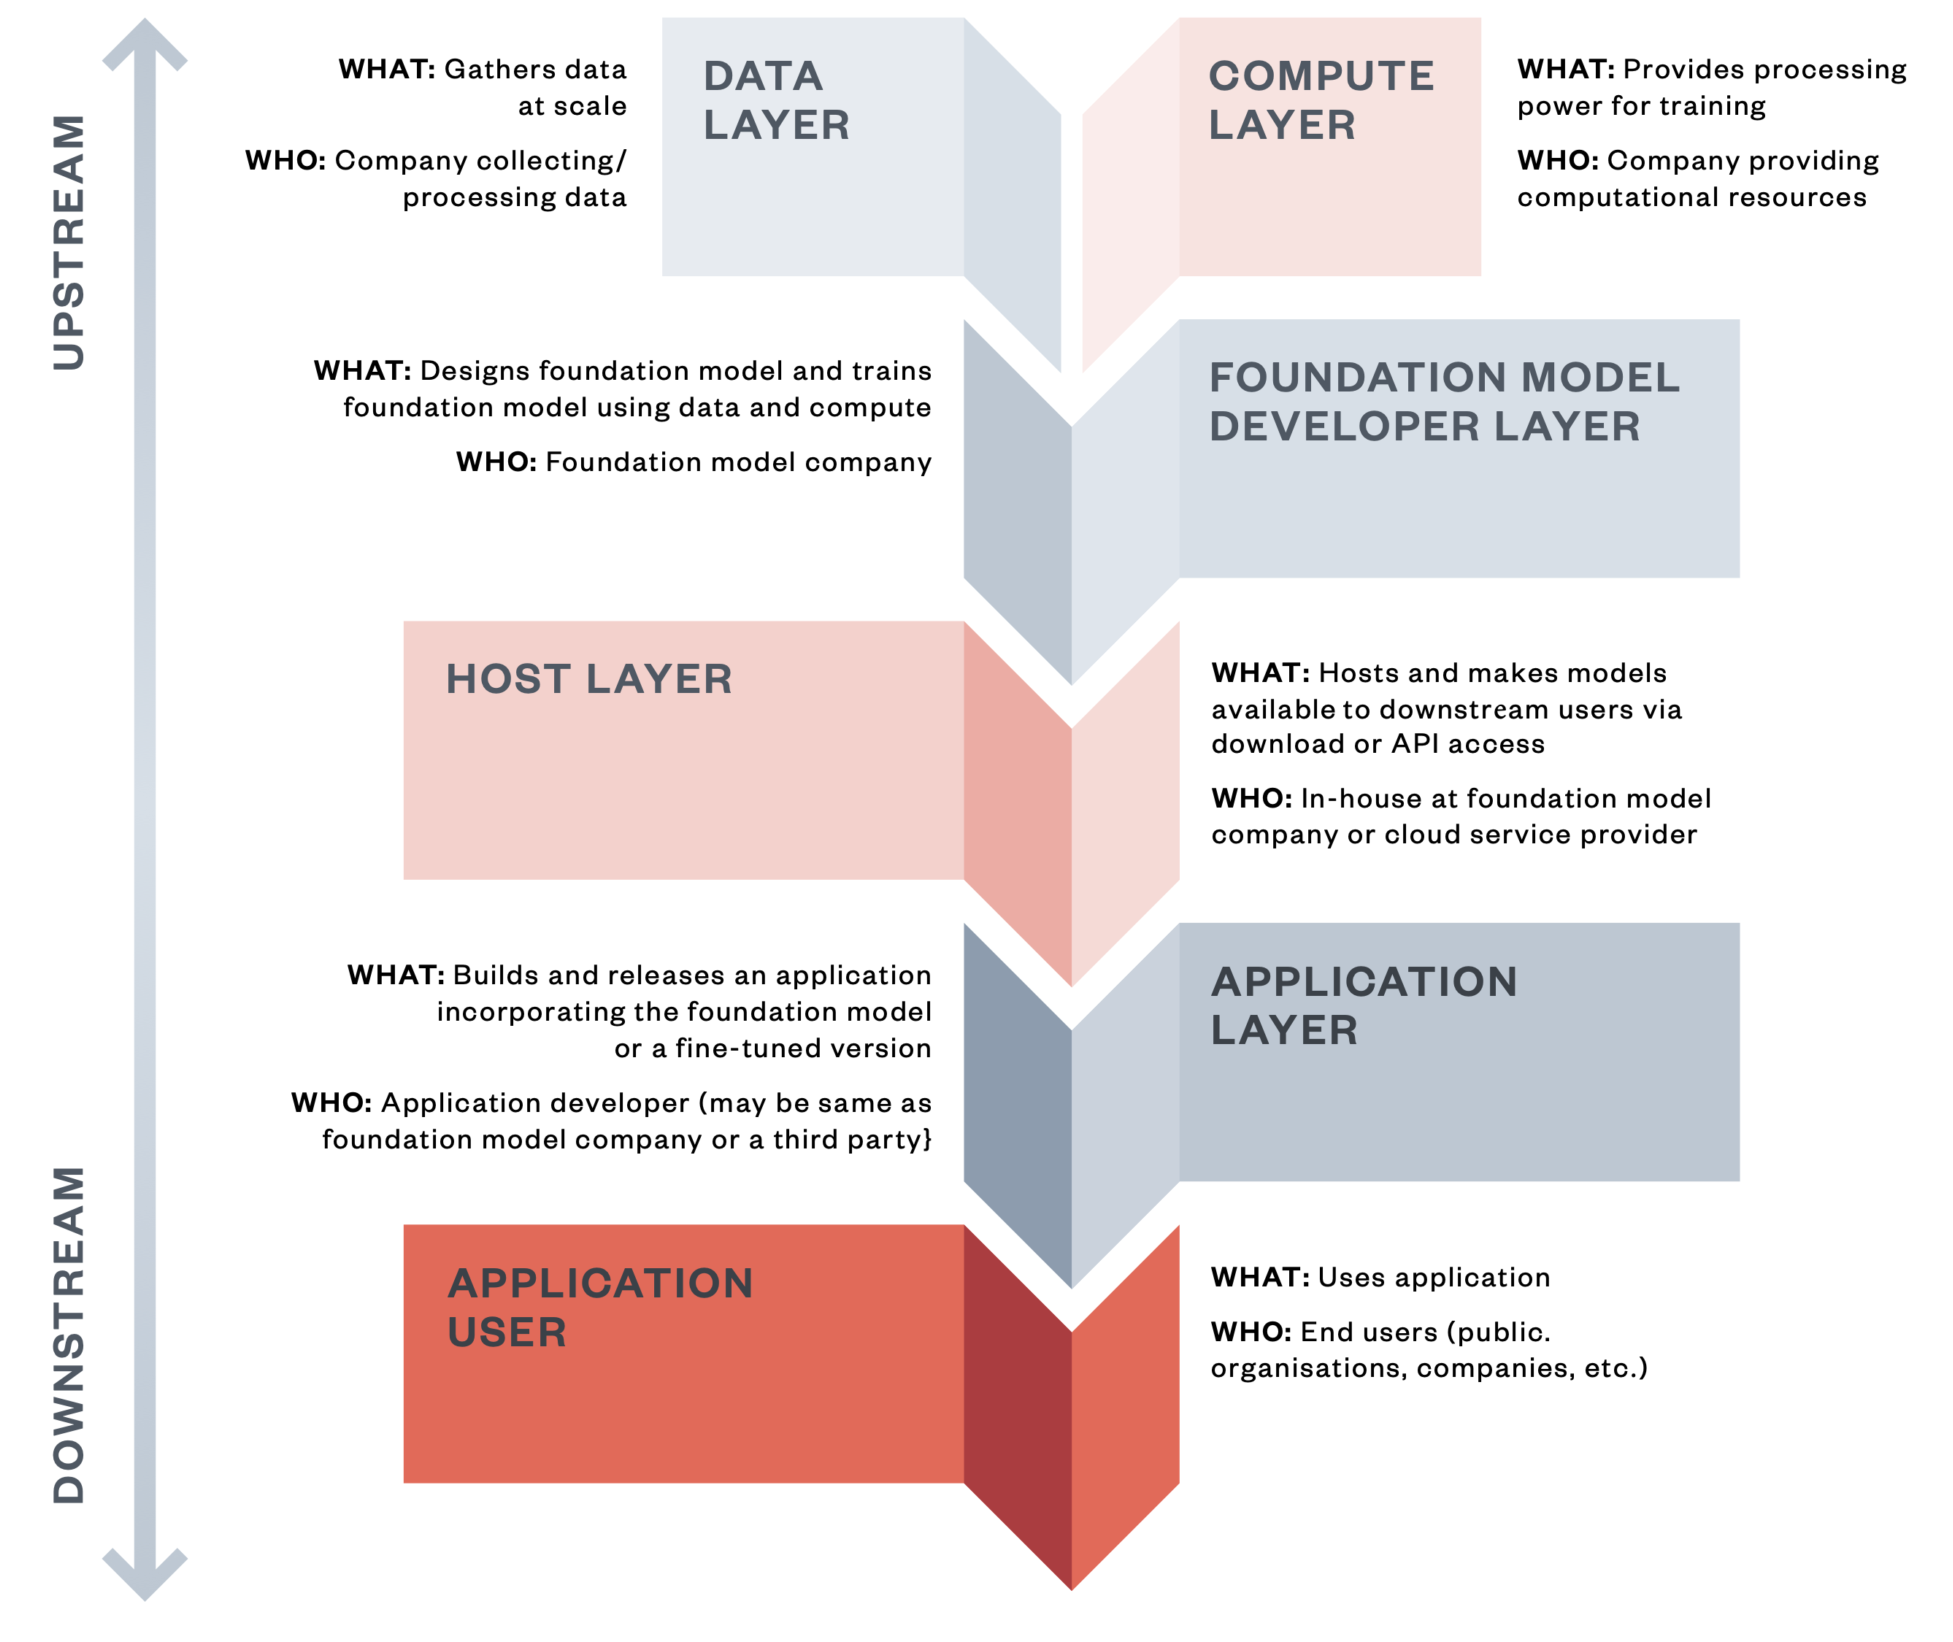
\includegraphics[width=\textwidth]{figures/supply_chain.png}
\caption{\textbf{Foundation Model Supply Chain.} 
A conceptual depiction of the foundation model supply chain, beginning with the primary \textit{upstream} resources (\ie data, compute) and transitioning to the foundation model, subsequent hosts (or \textit{distribution channels}), and ending with \textit{downstream} applications.
Image taken with permission from \citet{jones2023foundationmodels}.}
\label{fig:supply-chain}
\end{figure}

The structure of the foundation model paradigm implicates a broader ecosystem and supply chain \cite{bommasani2023ecosystem, cen2023supplychain, jones2023foundationmodels}.
We depict a conceptualized view of this supply chain in \reffig{supply-chain}.
The supply chain begins with the \textit{upstream} resources that are used to build a foundation model: data, computational hardware, energy, labor, and code. 
For each of these resources, a further supply chain exists: for example, data to build foundation models is often sourced from the Internet, but this data can only come to be on the Internet as a result of human data-generating process (\eg publishing news article, authoring personal blogs, uploading videos to YouTube, creating music) along with Internet infrastructure (\eg networking protocols).
Alongside these upstream resources and supply chains, foundation models are then used as the foundation for supply chains that derive from the model.
In particular, foundation models are made available for downstream use through \textit{distribution channels} (\eg an API to access the model or a host that facilitates inference using the model).
By way of these distribution channels, foundation models power \textit{downstream} applications (\eg commercial products and services) across a range of market sectors and geographies.
For instance, \openai's \gptfour powers applications in education (\eg Khan Academy's Khanmigo tutor), finance (\eg Stripe's fraud detection tool), banking (\eg Morgan Stanley's internal chatbot), and government (\eg Iceland's language preservation system).\footnote{See \url{https://openai.com/gpt-4} for a list of several applications built upon \openai's \gptfour.}
Overall, a comprehensive account of the societal impact of foundation models, and their transparency in particular, requires consideration of the different parts of the foundation model ecosystem \citep[][\S1.2]{bommasani2021opportunities}.

Foundation models have fueled the recent wave of generative AI technologies: these models can be used to generate fluent text, useful code, photorealistic images, and compelling audio.
New research efforts built foundation models in an even broader array of domains: biology \citep{lin2023evolutionary}, climate change \citep{lacoste2023geobench}, weather,\footnote{\url{https://www.earthdata.nasa.gov/news/weather-ai-fm-workshop}} astronomy \citep{nguyen2023astrollama}, radiology \citep{chambon2022roentgen}, and robotics \citep{openx2023openx}.
Nevertheless, much of the present public and commercial interest centers on language models (\eg \anthropic's \claude, \meta's \llama) and multimodal models with language interfaces (\eg \stability's \stablediffusion, \openai's \gptfour). 
Alongside their significant capabilities, researchers have highlighted a large number of potential risks posed by these foundation models spanning malicious uses like generating disinformation to unintended harms like generating text that reinforces societal biases \citep{bender2021dangers, bommasani2021opportunities, abid2021persistent, weidinger2022taxonomy}.
There have also been recent demonstrations of many concrete harms from language models.\footnote{Partnership on AI's AI Incident database (\url{https://incidentdatabase.ai/}) and the AI, Algorithmic, and Automation Incidents and Controversies database (\url{https://www.aiaaic.org/aiaaic-repository}) collect incidents of harm caused by AI. For a concrete example, see \url{https://www.404media.co/inside-the-ai-porn-marketplace-where-everything-and-everyone-is-for-sale/}.} 

\hypertarget{transparency}{\subsection{Transparency}}
\label{sec:background-transparency}
Transparency is broadly understood as the property of being visible and easily understood \citep{aristotle350deanima, kalderon2015transparency}, and is often a fundamental prerequisite of social responsibility and accountability \citep{florini2007right,robinson2012nations}.

Transparency is desirable from a variety of standpoints.
For example, transparently disclosing information makes that information available, shareable, legible, and verifiable. 
Transparency when conducting a complex process can make clear the processes' scope, stakes, and pitfalls \citep{lathrop2010open}. 
Similarly, transparency in decision-making can help those who are not involved in the decision assess the motivations behind the decision, the evidence used to justify it, as well as its costs and benefits.
Various philosophers, political theorists, scientists, and journalists have emphasized the importance of transparency across these and other domains \citep{johnston2006good,florini2007right, benkler2013practical, schudson2015rise}. 
Civil society, grassroots organizations, and consumers also regularly call for transparency as a mechanism for fact finding, accountability, and holding organizations responsible for harm \citep{heikkila2023high,diresta2022openblackbox}.\footnote{See \refapp{transparency} for additional details on calls for transparency.}
For our purposes, we consider transparency as it relates to the development and use of digital technologies, with a specific focus on the transparency of the practices of foundation model developers as measured by the information they share regarding their models.\footnote{Note that the term "transparency" is at times also used to describe efforts to make AI more explainable or interpretable at the level of specific AI-based predictions or decisions \citep{liao2023transparency, zou2023representation}. 
Such transparency is not the subject of our work.} 

\paragraph{Why transparent matters for digital technologies.}
Transparency in digital technologies is particularly relevant for three reasons.
First, new digital technologies, such as AI, are not well understood by society, often appearing as a black box \citep{castelvecchi2016openblackbox}. 
Second, digital technologies are easily rendered invisible, meaning it is difficult for nonexperts to understand when processes like algorithmic decision-making are taking place \citep{ng_conceptualizing_2021}.
Third, these technologies can have a profound influence on billions of users across society.
And yet these technologies are built by a small cadre of industry actors who do not represent society as a whole.
Under these conditions, transparency functions as a prerequisite for public accountability and responsible innovation \citep{klyman2023open}.
Shared visibility engenders public trust and facilitates interventions in the public interest \citep{hardin2002trust}. 
Without sufficient understanding of industry practices, researchers cannot characterize the societal impact of digital technologies, let alone propose concrete actions to improve business practices \citep{pasquale2015black}.
While the effects of transparency are often difficult to measure as they are diffuse and indirect, transparency helps to expose malpractice and enables the public to respond to such malpractice.

\paragraph{Limitations of transparency.} 
Transparency is far from sufficient on its own and it may not always bring about the desired change \citep{corbett2023interrogating}. 
Salient critiques of transparency include:
\begin{itemize}\itemsep0em
    \item Transparency does not equate to responsibility. Without broad based grassroots movements to exert public pressure or concerted government scrutiny, organizations often do not change bad practices \citep{boyd2016algorithmic,ananny2016limits}.
    \item Transparency-washing provides the illusion of progress. 
    Some organizations may misappropriate transparency as a means for subverting further scrutiny. 
    For instance, major technology companies that vocally support transparency have been accused of \emph{transparency-washing}, whereby "a focus on transparency acts as an obfuscation and redirection from more substantive and fundamental questions about the concentration of power, substantial policies and actions of technology behemoths" \citep{zalnieriute2021transparency}.
    \item Transparency can be gamified. Digital platforms have been accused of performative transparency, offering less insightful information in the place of useful and actionable visibility ~\citep{doi:10.1177/20539517231164119, Mittelstadt2019}. 
    As with other metrics, improving transparency can be turned into a game, the object of which is not necessarily to share valuable information.\footnote{According to Goodhart's Law, "when a measure becomes a target, it ceases to be a good measure" \citep{goodhart1984problems}.}
    \item Transparency can inhibit privacy and promote surveillance. 
    Transparency is not an apolitical concept and is often instrumentalized to increase surveillance and diminish privacy \citep{han2015transparency,Mohamed2020,birchall2021radical}. 
    For foundation models, this critique underscores a potential tension between adequate transparency with respect to the data used to build foundation models and robust data privacy.
    \item Transparency may compromise competitive advantage or intellectual property rights.
    Protections of competitive advantage plays a central role in providing companies to the incentives to innovate, thereby yielding competition in the marketplace that benefits consumers.
    Consequently, work in economics and management studies have studied the interplay and potential trade-off between competitive advantage and transparency \citep{bloomfield1999market, granados2013transparency, liu2023competitive}, especially in the discourse on corporate social responsibility \citep{}.
\end{itemize}

Transparency is not a panacea. 
In isolation, more information about foundation models will not necessarily produce a more just or equitable digital world. 
But if transparency is implemented through engagement with third-party experts, independent auditors, and communities who are directly affected by digital technologies, it can help ensure that foundation models benefit society.

\paragraph{Transparency in practice for prior digital technologies}
Digital technologies are marked by a long track record of poor transparency.
While each major new technology has dramatically restructured society, the powerful corporations that build these technologies have wielded outsized influence and maintained opacity to advance their commercial interests.
Consider the following examples of digital technologies that suffer from a lack of transparency as well as associated interventions/studies to reduce opacity:
the fight for net neutrality for internet service providers like Comcast \citep{crs2021netneutrality}, web cookies for online advertising like Google Ads \citep{englehardt2015cookies,englehardt2016online,narayanan2017princeton}, labor practices for crowd-sourcing platforms like Amazon Mechnical Turk \citep{gray2019ghost, crawford2021atlas}, wage schemes for ride sharing platforms like Uber \citep{rosenblat2016algorithmic}, and dark patterns for game companies like Epic Games \citep{ftc2023epicgames}.

Stepping through these examples, efforts like the Princeton Web Transparency Project \citep{englehardt2015cookies,englehardt2016online,narayanan2017princeton} have unveiled the ecosystem of online third-party tracking using cookies, which ``led to greater public awareness, the cessation of some privacy-infringing
practices, and the creation of new consumer privacy tools.''
Similarly, \citet{rosenblat2016algorithmic} empirically demonstrated that Uber drivers were the subject of a severely asymmetric power dynamic given the control exerted by Uber over their drivers, to the detriment of the ride sharing market.
In the context of crowd-sourcing, \citet{gray2019ghost} and \citet{crawford2021atlas} demonstrated exploitation of the ``ghost" workers powering AI, such as on Amazon Mechanical Turk, that was made invisible on these platforms.
More recently, these efforts have prompted the scrutiny of lawmakers as to improve transparency and, thereby, labor conditions.
As a final example, dark patterns have a pervasive practice for myriad technologies, leading to mismanaged consumer expectations and overall opacity. 
To this end, the FTC's recent inquiry into Epic Games for dark patterns used to deceive gamers, and particularly children, amounted to a \$245M fine on Epic Games \citep{ftc2023epicgames}.

Building on these prior examples, we consider social media more specifically.
Social media platforms provide a vivid example of transparency challenges in recent years, and the increasing level of acknowledgement among some technology companies that a baseline level of transparency is a necessity. 
Given the profound impact of social media in mediating how humans form relationships, communicate with each other, buy goods and services, and access information, a broad body of work argues for greater transparency \citep[see][]{keller2022platform}. 
Social media platforms have slowly begun to adopt transparency reporting practices.
For example, Facebook now hosts its own Ad Library\footnote{\url{https://www.facebook.com/ads/library/}}, Content Library\footnote{\url{https://transparency.fb.com/researchtools/meta-content-library}}, and a transparency center\footnote{\url{https://transparency.fb.com/}} that reports on content enforcement, widely viewed content, regulatory transparency, government data requests, and intellectual property, among other pieces of mostly voluntary transparency.
In parallel, transparency requirements have been enshrined in laws like the EU Digital Services Act \citep{dsa2022} and legislative proposals like the U.S. Platform Accountability and Transparency Act \citep{pata2021}. 

\paragraph{Transparency for AI.}
With the rise of AI in the past 10 years, its societal impact has received much greater attention \citep{barocas2016, abebe2020roles, hutchinson2021towards, bender2021dangers}.
Transparency is often referenced as a core ethical principle undergirding responsible AI \citep{fjeld2020principled, Hagendorff2020}.\footnote{See UNESCO's Recommendation on the Ethics of Artificial Intelligence, which was adopted by its 193 member states and constitutes the first global normative instrument on AI ethics. Our conceptualization of transparency covers several of UNESCO's 10 principles, namely Transparency and Explainability. See \url{https://www.unesco.org/en/artificial-intelligence/recommendation-ethics}} 
\citet{jobin2019global} find that transparency is the most frequently cited principle in AI ethics guidelines, appearing in 85\% of the assessed 84 guidelines. 

Given that the standard machine learning pipeline is divided into several stages, transparency efforts often target different stages.\footnote{As mentioned previously, the term "transparency" is also sometimes used in AI to refer to explainability/interpretability, referring to understanding how a specific model makes predictions \citep{zou2023representation}.
In part, the emphasis on this topic is due to the inscrutability of the deep neural networks that have powered AI's rise.
However, we focus on structural forms of transparency, taking a more macroscopic perspective.}
Documentation efforts are most common at the level of data \citep{gebru2021datasheets, bender2018data, pushkarna2022data} and models \citep{mitchell2018modelcards, crisan2022interactive}, with evaluations providing further insight into models \citep{deng2009imagenet, ribeiro2020beyond, perez2022red, liang2022helm, bommasani2023transparency}.
More recently, several efforts have studied the broader ecosystem-wide transparency of AI and its supply chains \citep{bommasani2023ecosystem, cen2023supplychain}, though transparency on the downstream impacts of AI is comparatively understudied \citep{narayanan2023transparencyreports}.
The \projectname advances this view, assessing transparency of foundation models with a comprehensive ecosystem-level approach that spans the data and broader upstream resources, the foundation models themselves, and the downstream use and impact.

\hypertarget{index}{\subsection{Indexes}}
\label{sec:background-index}
A (composite) index is a standard methodology \citep{oecd2008handbook, greco2019methodological} for assessing entities (\eg companies, countries) in relation to a specific construct (\eg transparency, responsibility).
Methodologically, the score on an index for a specific entity is the aggregate of multiple low-level indicators that can be more directly quantified. 
Composite indexes as a methodology has seen broad adoption across the social sciences, including to directly address major political, economic, and societal concerns such as public corruption \citep[\eg Transparency International’s Corruption Perceptions Index;][]{ti2022corrupt}, environmental welfare \citep[\eg the World Economic Forum’s Environmental Sustainability Index;][]{whitford2009political} and living standards \citep[\eg the United Nations Development Programme’s Human Development Index;][]{hopkins1991human}. 
However, indexes have not played a major role in mainstream AI discourse.\footnote{We highlight the AI Index from the Stanford Institute for Human-Centered AI \citep{maslej2023ai, zhang2022ai}, which tracks global progress of AI across a variety of quantitative indicators. 
In contrast to the composite indexes here, the AI Index neither directly scores specific entities nor does it aggregate individual indicators into a singular aggregate.
We also highlight the Generative AI Accountability Scorecard from Ranking Digital Rights as a forthcoming effort that targets the generative AI services downstream of foundation models: \url{https://rankingdigitalrights.org/mini-report/introducing-rdrs-preliminary-standards-for-generative-ai/}.
}

Indexes are designed to further several objectives and have certain characteristic strengths \citep{joint2008handbook, saisana2002state}. 
Most fundamentally, indexes can transform complex and amorphous constructs into straightforward and concrete scores.
Indexes and the aggregate quantitative metrics they provide can therefore allow for broad engagement on certain topics, furthering public understanding as well as providing a strong basis for various forms of decision-making  such as regulatory intervention. 
In addition, when indexes are maintained over time, they encourage a long-term focus and can be vital in fostering improvement over time.
In this way, while operating at a different level of abstraction and involving a different set of design decisions, indexes are analogous to model benchmarks that are commonplace in AI \citep{deng2009imagenet, wang2019superglue, liang2023holistic} and appeal to a similar theory of change \citep{donoho2017fifty, ethayarajh2020utility, raji2021benchmark, bommasani2022evaluation}.
Indexes also have shortcomings: namely, they can be reductive and overly subjective \citep{saisana2002state, oecd2008handbook, greco2019methodological}.
To design and score an index, researchers must make simplifying decisions about which indicators to include, how to weigh those indicators, and how to grade indicators.
Beyond these methodological issues, indexes are subject to a broader conceptual critique that they may oversimplify concepts that are intrinsically complex, discarding valuable nuances.\footnote{The literature and theory on composite indexes is much too extensive to be easily summarized in this brief primer.
We recommend the Handbook on Constructing Composite Indicators: Methodology and User Guide \citep{oecd2008handbook} as a proper introduction to the subject: \url{https://doi.org/10.1787/9789264043466-en}.} 
Indexes may also be subject to gaming, which we discuss more extensively in \refsec{limitations}.
\clearpage

\hypertarget{fmti}{\section{The Foundation Model Transparency Index}}
\label{sec:fmti}
The \projectname scores foundation model developers for their comprehensive transparency. 
We discuss specifics on the developers, indicators, and scoring in subsequent sections.
Strategically, our aim is for the index to clarify discourse on foundation models and AI that is muddled and lacks grounding in empirical data. 
We aim to improve the overall transparency of the AI ecosystem by encouraging foundation model developers to share more information about the development and deployment of their models. 
We also provide a clear taxonomization of the key issues related to transparency and demonstrate where greater transparency would be especially valuable. 
Therefore, the \projectname provides a frame of reference for assessing whether the ecosystem as a whole---and which developers in particular---become more or less transparency over time.
Simultaneously, given the limitations of indexes, we are fully transparent about our methodology, including the core decisions on indicator inclusion, indicator weighting, and indicator scoring.
We also discuss methodological shortcomings relating to each of these decisions in \refsec{limitations}.
To guard against unnecessary simplification, we provide discussion and analysis at several levels of abstraction in \refsec{results}. 

Overall, the \projectname captures the key dimensions of transparency that are relevant to foundation models at present.
As the foundation model ecosystem and AI policy evolves over time, the central questions regarding the transparency of foundation models will evolve as well.
Consequently, we will conduct future versions of the index that adjust the indicators to reflect these changes.
We more expansively discuss our intended impact (including our theory of change and associated limitations and risks) in \refsec{impact}.